%\documentclass[conference, twoside]{IEEEtran}
\documentclass[conference]{IEEEtran}
\IEEEoverridecommandlockouts
% The preceding line is only needed to identify funding in the first footnote. If that is unneeded, please comment it out.
%Template version as of 6/27/2024

\usepackage{multirow}
\usepackage{booktabs}
\usepackage{cite}
\usepackage{algorithmic}
\usepackage{graphicx}
\usepackage{textcomp}
\usepackage{xcolor}
\usepackage{amsmath,amsxtra,amssymb,amsthm,latexsym,amscd,amsfonts}
\usepackage[utf8]{vietnam}
\usepackage[english]{babel} %Figure ... English (có thể bỏ đi nếu bài viết tiếng Việt)
\usepackage{fancyhdr}
\pagestyle{fancy}

\renewcommand{\headrulewidth}{0pt} % dòng kẻ
\renewcommand{\footrulewidth}{0pt}
\renewcommand{\sectionmark}[1]{\markright{\MakeUppercase{#1}}{}}

% Trang lẻ (odd pages - thường ở bên phải khi lật sách)
\setlength{\oddsidemargin}{0.5pt}   % giảm lề trái
\addtolength{\textwidth}{-0.5cm}    % tăng lề phải

% Trang chẵn (even pages - thường ở bên trái)
%\setlength{\evensidemargin}{-0.5cm} % giảm lề trái hơn nữa
%\addtolength{\textwidth}{-0.5cm}      % tăng lề phải

\def\BibTeX{{\rm B\kern-.05em{\sc i\kern-.025em b}\kern-.08em
    T\kern-.1667em\lower.7ex\hbox{E}\kern-.125emX}}

%%% Edited 9/2/2025 by Phi Ho Truong
%\makeatother

\makeatletter
\def\ps@IEEEtitlepagestyle{%
\def\@oddhead{\hfil \small{\textit{Hội thảo khoa học Quốc gia về Trí tuệ nhân tạo (FJCAI) - Cần Thơ, 27-28/3/2026}\hfil}%
	\def\@evenhead{\hfil\small{\textit{Hội thảo khoa học quốc gia về Trí tuệ nhân tạo (FJCAI) - Cần Thơ, 27-28/3/2026}\hfil}}%
		\def\@oddfoot{\scriptsize \thepage \hfil }%
		\def\@evenfoot{\scriptsize \hfil \thepage}
	}
}
\makeatother

\makeatletter % changes the catcode of @ to 11
\newcommand{\linebreakand}{%
  \end{@IEEEauthorhalign}
  \hfill\mbox{}\par
  \mbox{}\hfill\begin{@IEEEauthorhalign}
}
\makeatother % changes the catcode of @ back to 12

\fancyhf{}
%\setcounter{page}{1}
%\fancyfoot[LE,RO]{\thepage}

\begin{document}
	
\fancyhead[RE,LO]{\centering{\small{\textit{Hội thảo khoa học Quốc gia về Trí tuệ nhân tạo (FJCAI) - Cần Thơ, 27-28/3/2026}}}}

% \title{Bản định dạng mẫu IEEEtran.cls dùng cho Hội thảo FJCAI có hỗ trợ mã tiếng Việt*\\
% {\footnotesize \textsuperscript{*}Note: Sub-titles are not captured for https://ieeexplore.ieee.org  and
% should not be used}
% \thanks{Identify applicable funding agency here. If none, delete this.}
% }
\title{Adaptive STEM Learning Pathway Optimisation via Reinforcement Learning}

\author{
    \IEEEauthorblockN{1\textsuperscript{st} Nhu-Tai Do}
    \IEEEauthorblockA{\textit{Dept. of Information Technology} \\
    \textit{Saigon University, Vietnam}\\
    Ho Chi Minh City, Vietnam \\
    dntai@sgu.edu.vn}
    
    \and
    \IEEEauthorblockN{2\textsuperscript{st} Nguyen Huu Loc}
    \IEEEauthorblockA{\textit{Dept. of Information Technology} \\
    \textit{Saigon University, Vietnam}\\
    Ho Chi Minh City, Vietnam \\
    lockbkbang@gmail.com}
    
    \and
    \IEEEauthorblockN{3\textsuperscript{st} Van Tuan Kiet}
    \IEEEauthorblockA{\textit{Dept. of Information Technology} \\
    \textit{Saigon University, Vietnam}\\
    Ho Chi Minh City, Vietnam \\
    vankiet27012004@gmail.com}    
    \and

    \linebreakand %
    \IEEEauthorblockN{4\textsuperscript{st} Nguyen Thi Ngoc Thanh}
    \IEEEauthorblockA{\textit{Dept. of Information Technology} \\
    \textit{Ho Chi Minh City Open University, Vietnam}\\
    Ho Chi Minh City, Vietnam \\
    thanh.ntn@ou.edu.vn}\thanks{Corresponding author: thanh.ntn@ou.edu.vn}    
}

\maketitle

\begin{abstract}
In the context of education 4.0, conventional learning management systems often lack effective personalization mechanisms, typically enforcing a uniform learning path for all learners. To address this limitation in STEM education, this paper proposes an adaptive learning framework based on the Q-learning algorithm, integrated into the Moodle platform via the LTI 1.3 standard. The learning process is modeled as a Markov decision process, combined with behavioral clustering to construct a multidimensional learner state space. To mitigate data scarcity and the cold-start problem, we introduce a data-driven simulation strategy that preserves the distributional characteristics of real learner behavior. Experimental results from 500 simulation iterations demonstrate that the proposed approach significantly outperforms traditional methods, achieving a 22.5\% improvement in average scores and a 51.0\% reduction in weak skills, thereby highlighting its potential for scalable, personalized STEM education.
\end{abstract}

\begin{IEEEkeywords}
Reinforcement learning, Q-learning, personalized learning, STEM education, data-driven simulation, Markov decision process
\end{IEEEkeywords}

%\IEEEpeerreviewmaketitle

\section{Introduction}
\label{sec:intro}

The rapid advancement of artificial intelligence is profoundly reshaping multiple domains, including education. According to the seminal study by Frey and Osborne, approximately 47\% of traditional occupations are at risk of automation \cite{frey2017future}, highlighting the urgent need to equip the workforce with new competencies, particularly in STEM. STEM education emphasizes the development of critical thinking and problem-solving skills; however, its effective implementation remains challenging due to the substantial heterogeneity in learners’ abilities, prior knowledge, and learning paces.

One of the most pressing challenges in contemporary education is the realization of large-scale personalized adaptive learning. Conventional learning management systems (LMS), such as Moodle and Blackboard, primarily function as repositories for learning materials and assessment records, offering limited capability for behavioral analysis and timely pedagogical intervention \cite{capuano2020adaptive}. In the Vietnamese context, existing studies on AI applications in education have predominantly focused on predictive tasks, such as forecasting dropout risks or final examination outcomes \cite{thuan2022ung, sang2020du}, while comparatively little attention has been paid to prescriptive approaches that actively recommend pedagogical actions to improve learning outcomes.

\begin{figure}[t]
    \centering
    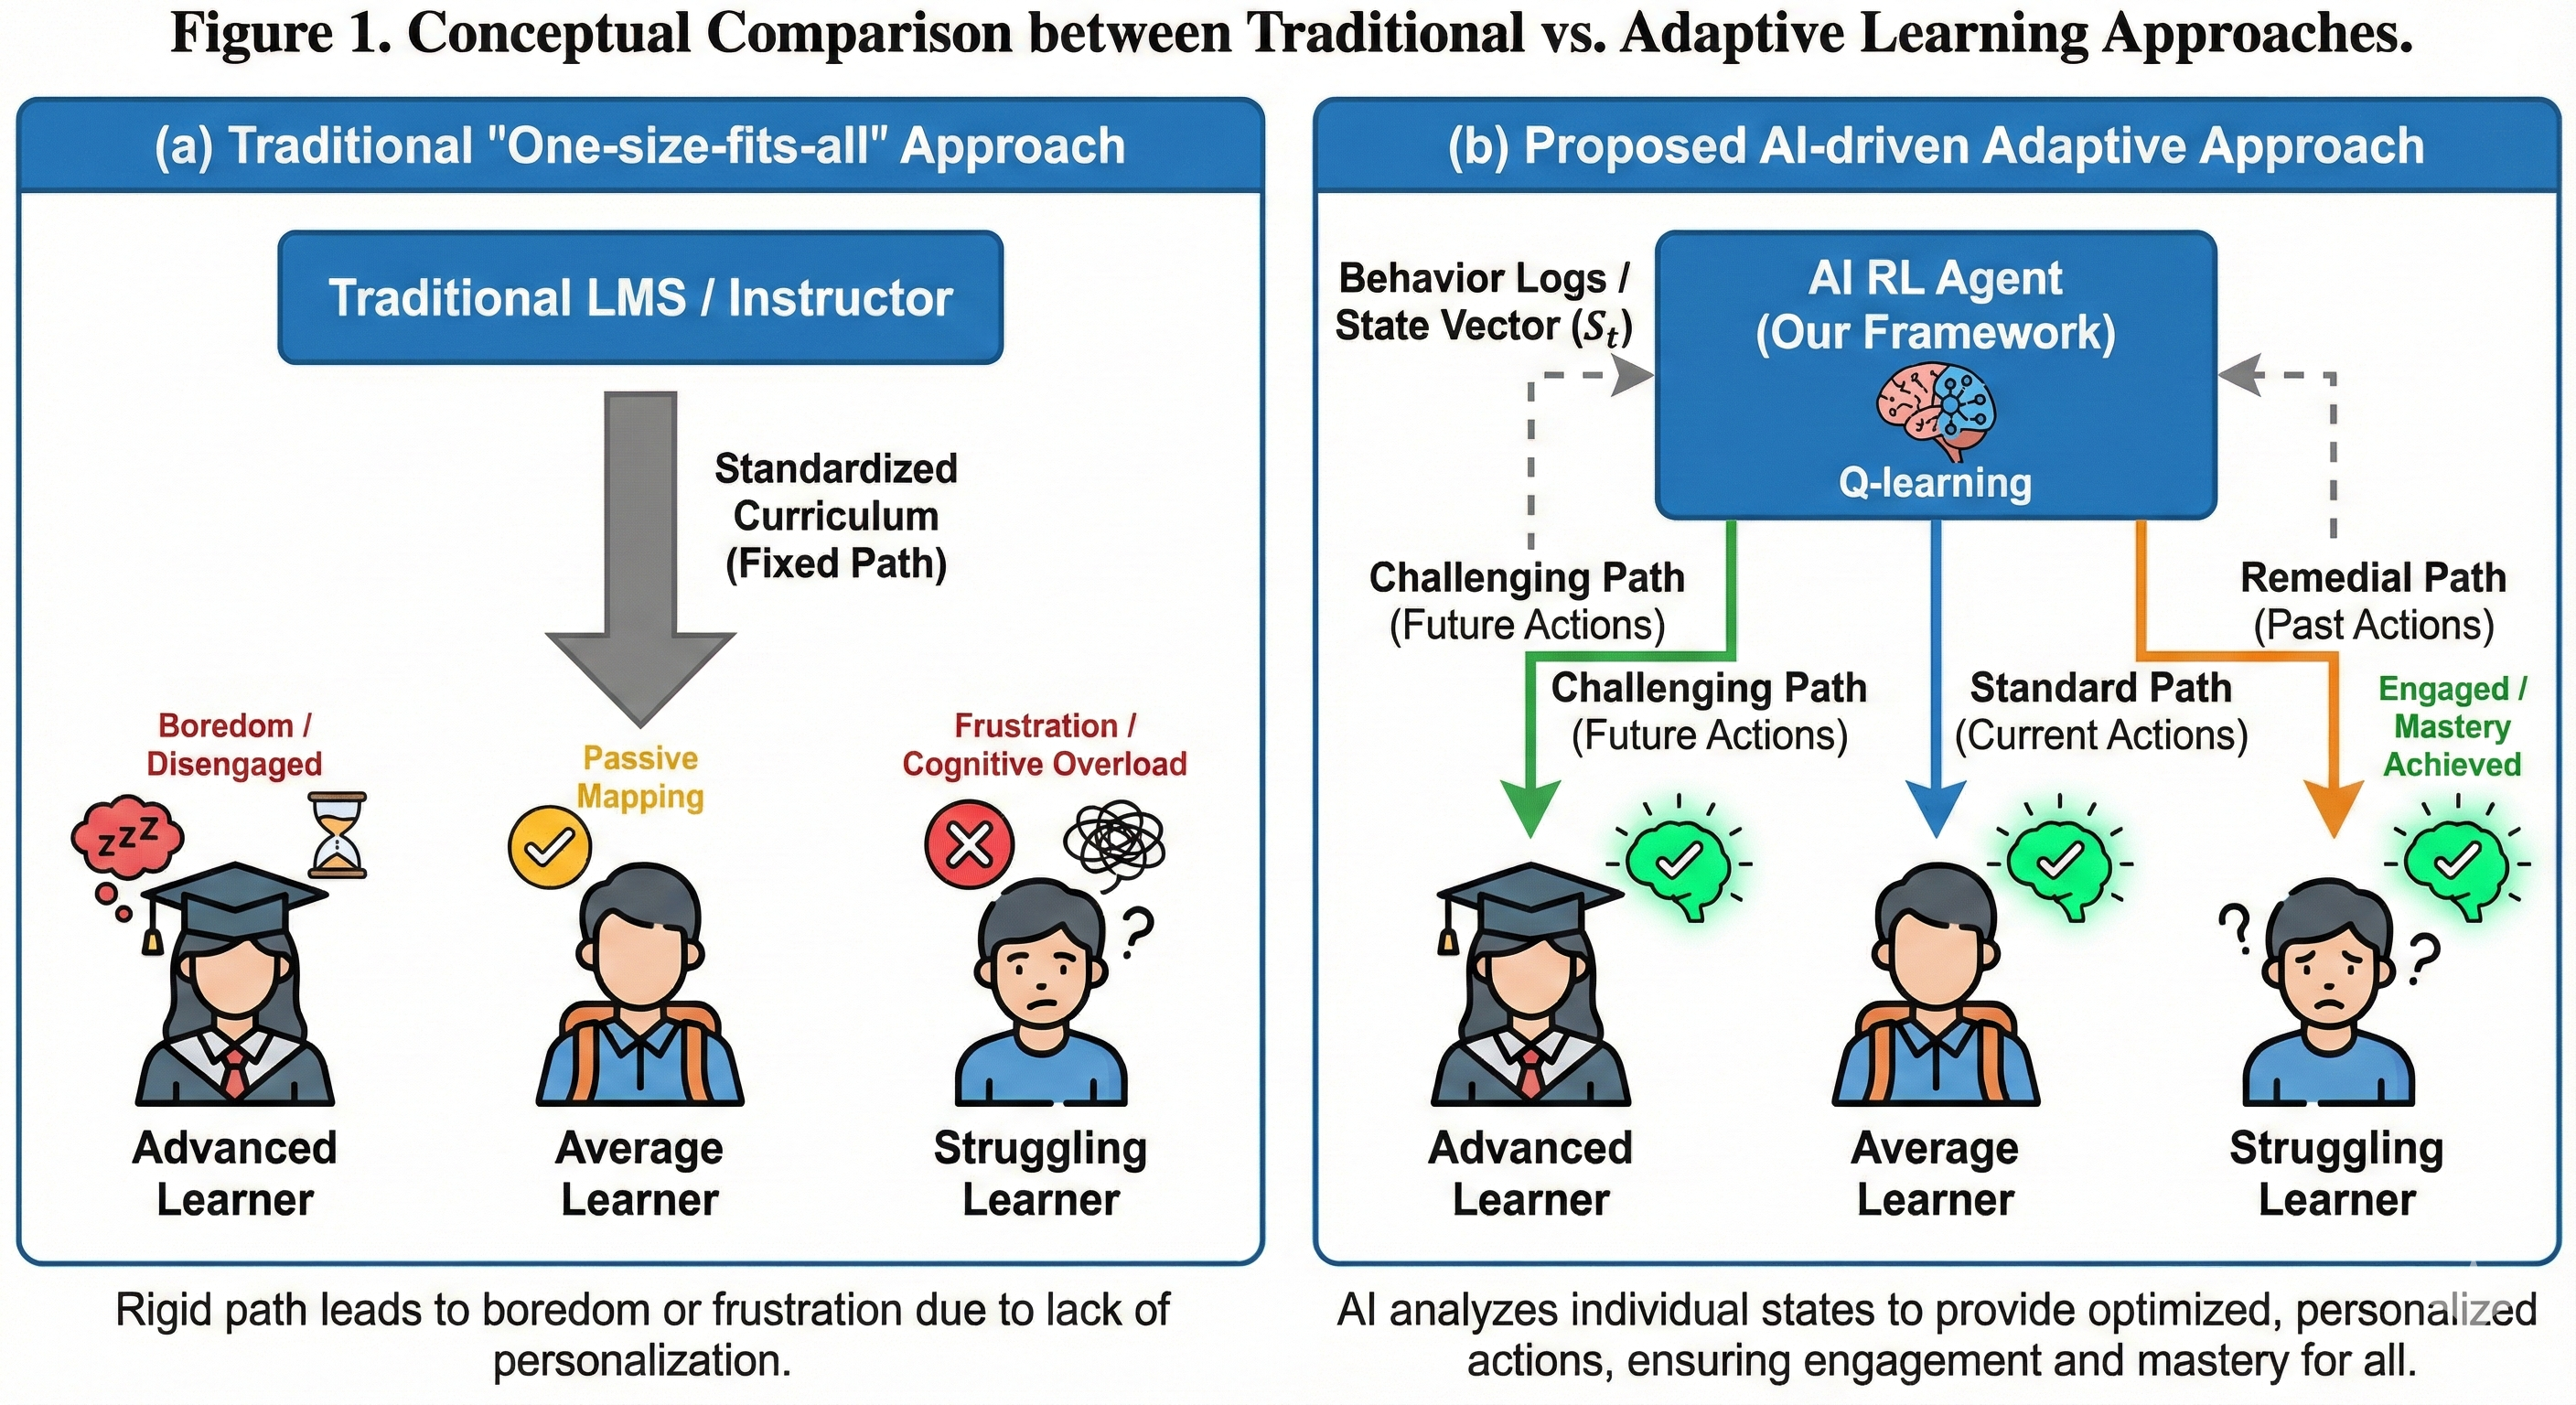
\includegraphics[width=0.9\linewidth]{fig1_problem_concept.pdf}
    \caption{Comparison of learning approaches. (a) Traditional methods apply a uniform learning path to all learners, often resulting in suboptimal engagement due to boredom or cognitive overload. (b) The proposed framework employs an AI agent to infer learner states from interaction logs and generate personalized action recommendations (review, standard, or enrichment) to maximize engagement and knowledge mastery.}
\label{fig:concept}
\end{figure}

To bridge this gap, there is a growing demand for personalized STEM teaching and learning support systems based on reinforcement learning (RL), as shown in Fig.\ref{fig:concept}. Unlike traditional rule-based systems, RL enables an intelligent agent to autonomously explore and optimize instructional strategies through a trial-and-error learning paradigm, continuously adapting its policy based on learner feedback and observed outcomes \cite{sutton1998reinforcement}.

\begin{figure}[t]
    \centering
    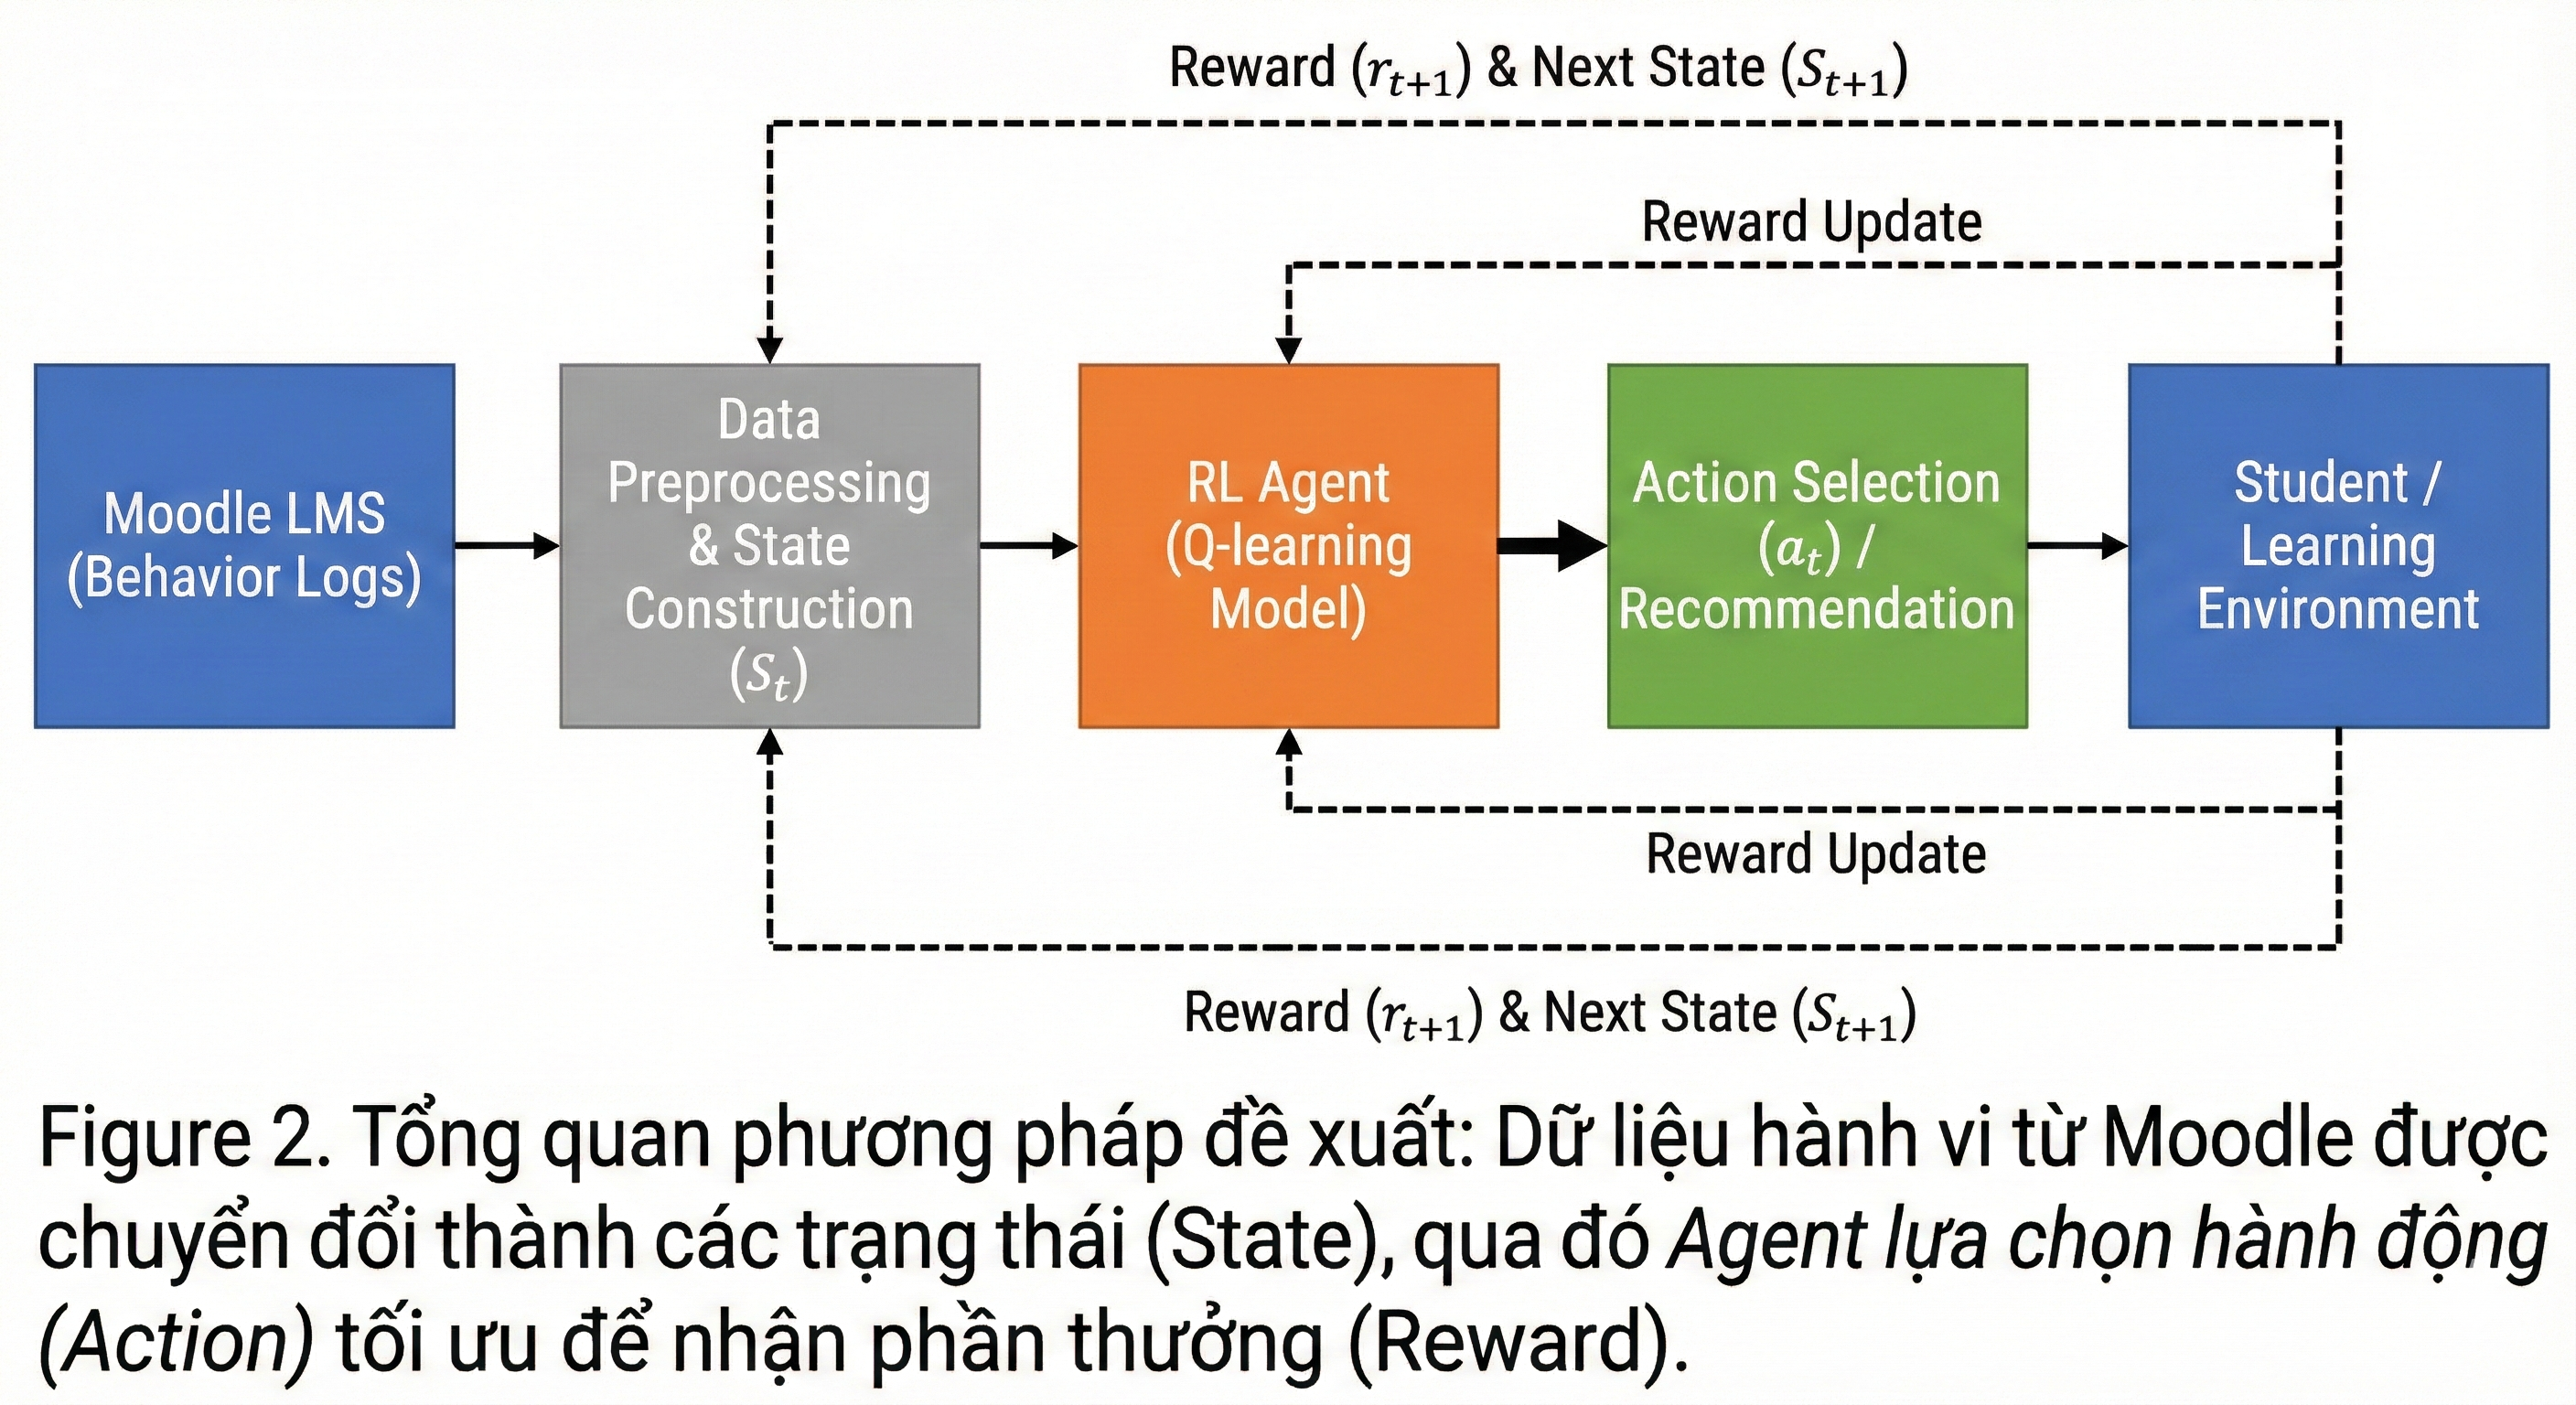
\includegraphics[width=0.8\linewidth]{fig2_method_overview.pdf}
    \caption{Proposed method overview. Moodle behavioral logs are transformed into learner states. Based on the current state, the agent selects an action and receives feedback in the form of rewards.}
    \label{fig:proposed_method}
\end{figure}

This study contributes to the field of personalized adaptive learning through the following three main aspects: (1) For the adaptive learning framework, we propose a reinforcement learning framework that models the learning process as a Markov Decision Process (MDP) with a multi-objective reward function. The framework integrates learner clustering results with behavioral learning theory, specifically the ICAP framework, to capture both cognitive engagement and performance-oriented objectives \cite{chi2014icap}; (2) With a data-driven simulation process, to address the challenges of data scarcity and the cold-start problem commonly encountered in educational settings, we design a data-driven simulation environment parameterized by statistical characteristics extracted from real course data, enabling a realistic approximation of learner behavior dynamics \cite{gligorea2023adaptive}; (3) About experimental validation, the effectiveness of the proposed approach is verified through A/B testing on a simulated dataset, where the Q-learning-based policy consistently outperforms traditional strategies in terms of academic performance and learner engagement, demonstrating its potential for scalable personalized STEM education.

\section{Proposed Method}
\label{sec:methodology}
\subsection{Problem Overview}
To overcome the limited personalization capabilities of conventional learning management systems, this study proposes an adaptive learning framework based on the Q-learning algorithm. The proposed pipeline starts from raw behavioral logs recorded by Moodle, applies preprocessing and feature engineering to construct a compact learner state space, and then trains an AI agent to select pedagogical actions that maximize long-term learning benefits. Fig.~\ref{fig:proposed_method} summarizes the overall workflow.

Personalized learning pathway recommendation is formulated as a MDP defined by the triplet $\langle S, A, R \rangle$, where $S$ denotes the state space, $A$ the action space, and $R$ the reward function.

\subsubsection{State Space $S$}
At time step $t$, the system observes the learner state $S_t$. To ensure generality and extensibility, we represent $S_t$ as a $d$-dimensional feature vector:
\begin{equation}
S_t = \{f_1, f_2, \ldots, f_d\}.
\end{equation}
In this study, the learner state is characterized by a compact yet informative feature set that captures both behavioral patterns and learning progress. Specifically, learners are first assigned to a behavioral cluster $C$ obtained through unsupervised clustering techniques. The current learning context is represented by the module index $M$ and the corresponding completion level $P$. Academic performance is summarized by a discretized cumulative score level $Sc$. In addition, the learning process is contextualized by the learning phase $Ph$, aligned with the ICAP framework, and by the engagement level $E$, which reflects the intensity and quality of learner interactions derived from activity logs.

\begin{figure}[t]
    \centering
    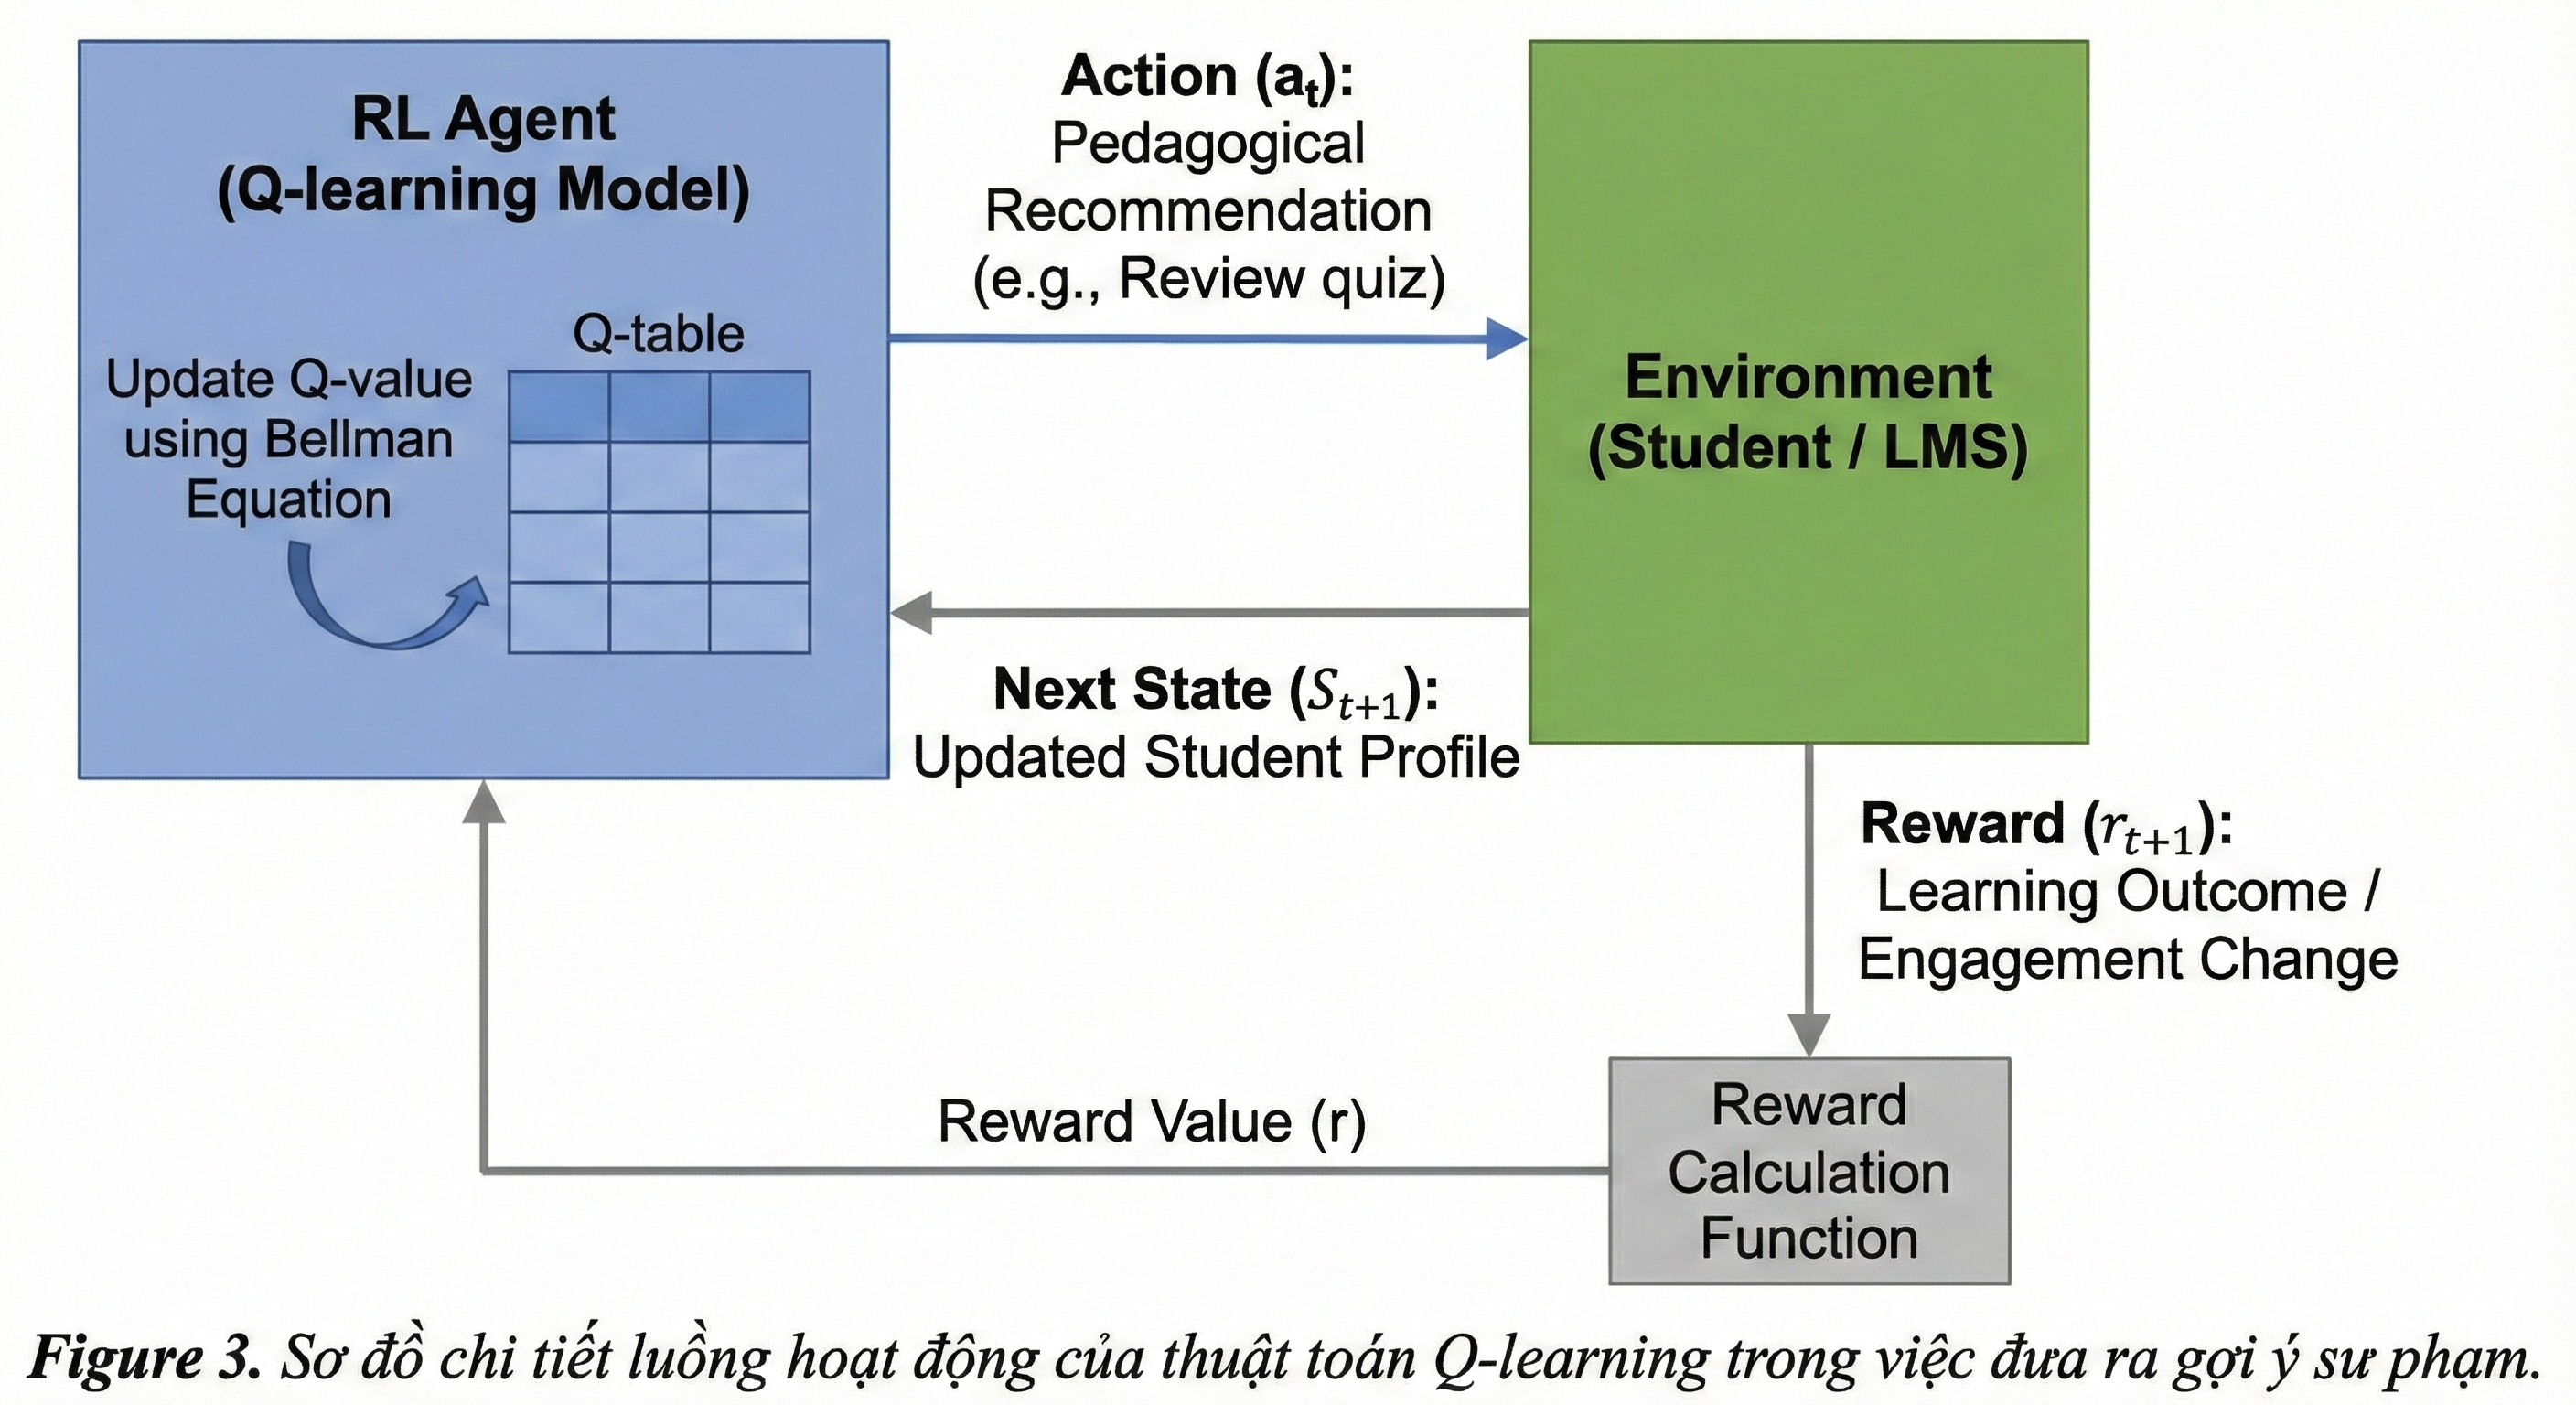
\includegraphics[width=0.9\linewidth]{fig3_qlearning_diagram.pdf}
    \caption{Detailed flowchart of the Q-learning procedure for generating pedagogical recommendations.}
    \label{fig:qlearning_diagram}
\end{figure}

\subsubsection{Action Space $A$}
Given $S_t$, the agent chooses an action $a_t \in A$ from a finite set of $m$ pedagogical actions $A = \{a_0, a_1, \ldots, a_{m-1}\}$. Actions are organized along a temporal axis (past, present, and future) to support different instructional intents, including remedial review for struggling learners and enrichment for advanced learners.

\subsubsection{Reward Function $R$}
The objective is to maximize the accumulated reward over time. To reflect multiple pedagogical goals, we define a multi-objective reward:
\begin{equation}
R_{\text{total}} = R_{\text{base}} + R_{\text{LO}} + R_{\text{bonus}} - P_{\text{penalty}}.
\end{equation}
Here, $R_{\text{base}}$ provides a baseline incentive for meaningful engagement, $R_{\text{LO}}$ captures learning-outcome attainment, $R_{\text{bonus}}$ rewards beneficial behavior sequences, and $P_{\text{penalty}}$ penalizes inefficient or unproductive actions.

\subsection{Data Processing and Clustering}
Raw LMS logs are typically noisy and unstructured. Before being used by the RL agent, the logs are preprocessed (filtering, normalization, and feature extraction) to obtain a compact behavioral representation. We then apply K-means to partition learners into $K$ clusters with similar behavioral characteristics.

The optimal number of clusters is selected using three complementary validation criteria: the Elbow method (inertia), the Silhouette coefficient (inter-cluster separation), and the Davies-Davies–Bouldin (cluster compactness). A majority voting scheme aggregates the three criteria to determine the final $K$. The resulting cluster ID is incorporated as a key component of the state vector $S_t$.

\subsection{Q-learning Algorithm}
We adopt Q-learning to learn the optimal state and state-action function (Q-table) using Bellman’s update rule shown in Fig.\ref{fig:qlearning_diagram}:
\begin{equation}
Q(s, a) \leftarrow Q(s, a) + \alpha \left[r + \gamma \max_{a'} Q(s', a') - Q(s, a)\right],
\end{equation}
where $\alpha$ is the learning rate and $\gamma$ is the discount factor. An $\epsilon$-greedy strategy is employed to balance exploration and exploitation during training.

\subsection{Explainability Framework}
To mitigate the black-box nature of the learned Q-table, we integrate SHAP \cite{lundberg2017unified} to quantify how each state feature contributes to the agent’s decision.

\subsubsection{Mathematical Basis}
The SHAP value $\phi_i(s)$ measures the marginal contribution of feature $i$ to the predicted utility:
\begin{equation}
\phi_i(s) = \sum_{S \subseteq F \setminus \{i\}} 
\frac{|S|!(|F|-|S|-1)!}{|F|!}
\left[f(S \cup \{i\}) - f(S)\right].
\end{equation}
The additive property ensures:
\begin{equation}
f(s) = \phi_0 + \sum_{i=1}^{6} \phi_i(s).
\end{equation}
To assess global importance, we compute the mean absolute SHAP value over $N$ randomly sampled states:
\begin{equation}
I_i = \frac{1}{N}\sum_{j=1}^{N}|\phi_i(s_j)|.
\end{equation}

\subsubsection{KernelExplainer Implementation}
Shapley value approximation is performed in three steps:
\begin{enumerate}
    \item \textbf{Prediction function:} Define a wrapper function $f(s) = \max_{a} Q(s,a)$ that maps a state $s$ to its maximum expected utility.
    \item \textbf{Background sampling:} Use a background set $D_{\text{bg}}$ ($N_{\text{bg}}=100$) to approximate the baseline expectation $E[f(x)]$.
    \item \textbf{Computation:} For each test state, KernelExplainer evaluates all $2^6=64$ feature coalitions, yielding accurate attributions with a computational cost of $O(N \cdot 2^D)$.
\end{enumerate}

\subsection{Data-driven Simulation Framework}
To address the \textit{cold-start} issue and promote stable convergence before real deployment, we propose a \textbf{parameter mining} procedure that transforms historical logs into probabilistic parameters to operate a classroom \textit{digital twin}.

\subsubsection{Action Mapping and Contextualization}
Low-level Moodle events are normalized into a unified action space $A$ comprising 15 canonical actions. To refine decision context, each action is labeled with a temporal context derived from learner progress $P_t$:
\begin{equation}
Context(a_t) =
\begin{cases} 
\text{Past}, & \text{if } P_t < 25\%, \\
\text{Current}, & \text{if } 25\% \le P_t < 85\%, \\
\text{Future}, & \text{if } P_t \ge 85\%.
\end{cases}
\end{equation}

\subsubsection{Transition Dynamics Modeling}
Using historical data $\mathcal{D}_{history}$, we estimate a transition probability matrix (TPM) $\mathcal{P}$. For each state--action pair $(s, a)$, the probability of transitioning to the next state $s'$ is estimated by:
\begin{equation}
P(s' \mid s, a) = \frac{count(s, a, s')}{\sum_{s^*} count(s, a, s^*)}.
\end{equation}
The matrix $\mathcal{P}$ governs the simulated environment, ensuring that its responses are consistent with observed learner dynamics.

\subsubsection{Param Policy Baseline}
For benchmarking, we construct a \textbf{Param Policy} baseline $\pi_{\text{param}}$ from historical action frequency distributions, stratified by learning phase and learner cluster:
\begin{equation}
\begin{aligned}
\pi_{\text{param}}(a \mid s) &= P(a \mid \text{Phase}(s), \text{Cluster}(s)) \\
&= \frac{\text{count}\big(\text{Phase}(s), \text{Cluster}(s), a\big)}
        {\sum_{a'} \text{count}\big(\text{Phase}(s), \text{Cluster}(s), a'\big)}.
\end{aligned}
\end{equation}
This baseline mimics learners’ natural historical tendencies and serves as a reference point against the optimized Q-learning policy $\pi^*$.

\subsubsection{Training and Evaluation Procedure}
The simulation is executed in a closed-loop manner:
\begin{enumerate}
    \item \textbf{Initialization:} Instantiate student agents whose behavioral profiles are parameterized from cluster statistics.
    \item \textbf{Training:} The RL agent interacts with student agents in the environment $\mathcal{P}$ to optimize the Q-table via trial-and-error.
    \item \textbf{Comparison:} Evaluate and compare performance (Reward, Score, LO Mastery) between the learned policy $\pi^*$ and the baseline $\pi_{\text{param}}$.
\end{enumerate}

\section{Experiments and Results}
\label{sec:experiments}

\subsection{Simulation Setup}

\subsubsection{Learning Style Modeling}
Virtual student agents in the simulation are not assumed to behave randomly; instead, they are endowed with heterogeneous and non-linear learning styles in order to better approximate authentic classroom behavior. Based on empirical observations from the dataset, the population is configured with three dominant learning styles: the majority are linear learners (70\%), who follow a conventional sequential pathway by progressing through learning materials and activities in the prescribed order; a smaller group of practice-first learners (10\%), who prioritize attempting quizzes or exercises before engaging with theoretical content; and a group of video/reading-first learners (20\%), who prefer passive content consumption such as videos or readings prior to active interaction.

\subsubsection{Simulation settings and stochasticity}
To ensure objectivity and reproducibility, the simulation environment is configured with explicit control over scale, randomness, and termination conditions.

Scale and reproducibility: Training is conducted over 500 episodes. In each episode, a population of 100 virtual student agents is initialized, resulting in a total of 50{,}000 simulated interaction trajectories. This scale provides sufficient coverage of the discretized state space. All experiments use a fixed random seed of 42 to ensure reproducibility across runs.

Noise modeling: Stochastic components are incorporated to reflect variability in real-world learner behavior. Score variation $\sigma$ obtained after each action is perturbed by uniform noise to simulate performance fluctuations:
\begin{equation}
S_{\text{real}} = \text{clip}\left(S_{\text{base}} + \mathcal{U}(-\sigma_c, \sigma_c), 0, 1\right),
\end{equation}
where $\sigma_c$ denotes the variability characteristic of each learner group. The Weak group exhibits the highest variability ($\sigma = 0.18$), followed by the Medium group ($\sigma = 0.10$), while the Strong group shows the lowest variability ($\sigma = 0.05$).

Time variation required to complete an action is randomly sampled from a uniform distribution to capture differences in information processing speed:
\begin{equation}
T \sim \mathcal{U}(5, 30) \ \text{minutes}.
\end{equation}


Termination conditions: Each episode terminates when the learner agent completes all $N = 6$ modules of the course or when a maximum step limit of 100 is reached. This constraint prevents infinite loops during the early exploration phase of training.

\begin{table}[htbp]
\caption{Summary of simulation configuration parameters}
\label{tab:sim_params}
\begin{center}
\begin{tabular}{lp{4.5cm}c}
\toprule
\textbf{Parameter} & \textbf{Description} & \textbf{Value} \\
\midrule
$N_{\text{episodes}}$ & Number of training episodes & 500 \\
Seed & Random seed & 42 \\
$N_{\text{modules}}$ & Number of course modules & 6 \\
\midrule
\multicolumn{3}{l}{\textit{Cluster-dependent parameters:}} \\
$P_{\text{success}}$ (Weak) & Baseline success probability & 0.72 \\
$P_{\text{success}}$ (Medium) & Baseline success probability & 0.78 \\
$P_{\text{success}}$ (Strong) & Baseline success probability & 0.90 \\
$\alpha_{\text{learn}}$ (Weak) & Learning rate & 0.22 \\
$\alpha_{\text{learn}}$ (Medium) & Learning rate & 0.32 \\
$\alpha_{\text{learn}}$ (Strong) & Learning rate & 0.30 \\
\bottomrule
\end{tabular}
\end{center}
\end{table}

\subsection{Experimental Setup}

\subsubsection{Ground-Truth Dataset}
This study uses the publicly available \textit{Moodle Log \& Grades} dataset~\cite{dataset_kaggle}. Among the available courses, we selected \textbf{Course ID 670} as the empirical basis for constructing the data-driven simulation environment.

This choice is motivated by its balanced data characteristics. The course contains 13{,}995 interaction events from 23 students, with an approximately normal score distribution ($\mu = 7.64$, $\sigma = 2.95$). In contrast, several other courses exhibit highly skewed score distributions (e.g., Course ID 42 with a mean score of 1.07), which can obscure behavioral differences and hinder the learning agent’s ability to distinguish strategies across competency groups (e.g., Excellent, Average, and Weak). Therefore, Course ID 670 provides a reliable foundation for both clustering analysis and policy learning.

\subsubsection{Data Preprocessing and Clustering}
We apply K-means clustering due to its efficiency and suitability for numerical feature spaces shown in Fig.\ref{fig:clustering_metrics}. To improve robustness and avoid subjective parameter tuning, the clustering pipeline incorporates (i) a two-stage feature filtering procedure and (ii) a majority voting mechanism for selecting the optimal number of clusters.

\textbf{1) Feature selection and filtering:}
All numerical features are first standardized using Z-score normalization. We then refine the feature space using two complementary filters:
\begin{itemize}
    \item \textbf{Variance filtering:} Remove features with variance below 0.01, as such low-variability features provide limited discriminative power.
    \item \textbf{Correlation filtering:} Remove highly correlated features (Pearson correlation $> 0.95$) to reduce redundancy and mitigate multicollinearity. This step eliminates 78 duplicated features and stabilizes the clustering structure.
\end{itemize}

\textbf{2) Cluster optimization $K$:}
The number of clusters $K$ is determined by aggregating three validation criteria  shown in Fig.~\ref{fig:clustering_metrics}: the elbow method (inertia), the silhouette coefficient (separation), and the Davies-Bouldin index (compactness). The three criteria are combined via a majority voting rule.
\begin{itemize}
    \item \textbf{Elbow method:} The inertia curve exhibits a clear knee point at $K=6$.
    \item \textbf{Silhouette coefficient:} Peaks at $K=2$ (0.42) but remains acceptable at $K=6$ ($\approx 0.35$).
    \item \textbf{Davies–Bouldin index:} Shows a favorable local minimum at $K=6$ (lower is better).
\end{itemize}

\begin{figure}[t]
\centerline{\includegraphics[width=0.9\columnwidth]{fig4_clustering_metrics.pdf}}
\caption{Clustering validation metrics. The Elbow and Davies-Bouldin criteria indicate $K=6$, while the Silhouette coefficient remains acceptable at this value.}
\label{fig:clustering_metrics}
\end{figure}

\textbf{3) Rationale for choosing $K=6$:}
Although $K=2$ yields the highest Silhouette score, partitioning learners into only two groups (e.g., Excellent vs. Weak) is overly coarse and does not provide sufficient granularity for the agent to optimize differentiated pedagogical actions. Conversely, selecting a large number of clusters (e.g., $K \ge 10$) substantially increases complexity and leads to state-space explosion. Therefore, it $K=6$ offers a practical trade-off, capturing six representative learner competency profiles while remaining computationally tractable.

During the cluster inspection, one cluster was identified as corresponding to instructor behavior, characterized by a high frequency of grading-related and forum moderation events. This cluster was excluded from the training data. The remaining five student clusters are subsequently mapped into three pedagogical groups (weak, medium, and strong) to support adaptive reward shaping in later stages.

\subsubsection{Modeling transition dynamics and baseline}
The fidelity of the proposed simulation environment is governed by the transition probability matrix (TPM), which captures how learners evolve from one state to another in response to pedagogical actions. Transition probabilities are estimated from historical interaction data through detailed frequency analysis. The resulting probability distributions are organized into structured tables and subsequently used as input parameters for constructing the parametric baseline policy ($\pi_{\text{param}}$), which serves as a reference model of natural learner behavior.

\textbf{1) Action distribution across learning phases:}
Table~\ref{tab:phase_probs} summarizes the empirical distribution of learner actions across different learning phases. A clear progression in behavioral patterns can be observed: during the pre-learning phase, learners predominantly engage in passive activities (viewing assignments and content); in the active phase, behavior shifts toward constructive actions such as quiz attempts and assignment submissions; and in the reflective phase, interaction becomes exclusively discussion-oriented through forum posting.

\begin{table}[t]
\caption{Probability of action selection by learning phase}
\label{tab:phase_probs}
\begin{center}
\begin{tabular}{llc}
\toprule
\textbf{Phase} & \textbf{Action ($a_t$)} & \textbf{Probability ($P$)} \\
\midrule
\multirow{2}{*}{Phase 0 (Pre-learning)} & view\_assignment & 56.4\% \\ 
& view\_content & 43.6\% \\
\midrule
\multirow{2}{*}{Phase 1 (Active)} & \textbf{attempt\_quiz} & \textbf{74.4\%} \\ 
& submit\_assignment & 25.6\% \\
\midrule
Phase 2 (Reflective) & post\_forum & 100.0\% \\
\bottomrule
\end{tabular}
\end{center}
\end{table}

\textbf{2) Action distribution by engagement level:}
Table~\ref{tab:engage_probs} reports action selection patterns conditioned on learner engagement levels. Highly engaged learners exhibit a balanced strategy, alternating between content consumption and task completion. In contrast, learners with low engagement predominantly focus on viewing assignment requirements (\textit{view\_assignment}), indicating a more passive and preparatory interaction style.

\begin{table}[t]
\caption{Action probability distribution by engagement level}
\label{tab:engage_probs}
\begin{center}
\resizebox{\columnwidth}{!}{%
\begin{tabular}{lccccc}
\toprule
\textbf{Engagement Level} & \textbf{View Assign} & \textbf{View Content} & \textbf{Quiz} & \textbf{Submit} & \textbf{Forum} \\
\midrule
\textbf{High} & 52.2\% & 40.5\% & 5.8\% & 1.5\% & 0.02\% \\
\textbf{Medium} & 51.7\% & 41.9\% & 4.3\% & 2.2\% & -- \\
\textbf{Low} & \textbf{57.6\%} & 34.0\% & 4.8\% & 3.6\% & -- \\
\bottomrule
\end{tabular}
}
\end{center}
\end{table}

The extracted probability distributions are exported as structured JSON configurations and used to drive the stochastic yet directed behavior of virtual student agents during simulation. This design ensures that the baseline policy and transition dynamics closely mirror empirically observed learner behaviors, providing a realistic benchmark against which the reinforcement learning policy can be evaluated.

\subsubsection{Model Parameters}
To ensure stable learning dynamics and convergence of the Q-learning algorithm, the model parameters were carefully configured as follows.

\textbf{State Space ($S$):} The learner state at time $t$, denoted by $S_t$, is represented as a 6-dimensional contextual vector:
\begin{equation}
S_t = (C, M, P, Sc, Ph, E)
\end{equation}
where $C$ denotes the learner behavior cluster obtained from the K-means model with $K=6$. After excluding one cluster corresponding to instructor activity, the remaining five student clusters are encoded as $C \in \{0,1,2,3,4\}$.  
$M$ represents the current module index; $P$ and $Sc$ denote the learner’s progress and score level, respectively, both discretized into four ordinal levels.  
$Ph$ indicates the learning phase ($0$: pre-learning, $1$: active learning, $2$: reflective learning), while $E$ captures the engagement level (low, medium, high).  
Under this formulation, the total state space comprises $5 \times 6 \times 4 \times 4 \times 3 \times 3 \approx 4{,}320$ distinct states, balancing representational richness and computational tractability.

\textbf{Action Space ($A$):} The action space consists of $m=15$ pedagogical actions, selected based on the ICAP framework and filtered using a Pareto threshold ($>1\%$ occurrence frequency). For interpretability and policy design, actions are organized according to their temporal context (past, current, future), as summarized in Table~\ref{tab:action_space_compact}.

\textbf{Q-learning Hyperparameters:} The learning rate is set to $\alpha = 0.1$, and the discount factor to $\gamma = 0.95$. An $\epsilon$-greedy exploration strategy with a monotonically decreasing $\epsilon$ is employed to balance early-stage exploration and late-stage exploitation, thereby facilitating convergence toward an optimal policy.

\subsubsection{State Space Modeling}
The adaptive learning problem is formulated as a MDP, in which the learner state at time $t$ is represented by a compact yet expressive 6-dimensional vector that integrates both static learner characteristics and dynamic behavioral signals:
\begin{equation}
S_t = (C, M, P, Sc, Ph, E)
\end{equation}
Here, it $C$ denotes the learner behavior cluster, $M$ the current module index, $P$ the learning progress, $Sc$ the score level, $Ph$ the learning phase, and $E$ the engagement level. This joint representation enables the agent to capture not only where the learner is in the course structure but also how they are learning.

To guarantee tractable learning and ensure convergence of the Q-table under limited computational resources, all continuous variables are discretized using pedagogically motivated thresholds. The detailed definitions and value domains of each state component are summarized in Table~\ref{tab:state_space_detail}. This discretization strategy strikes a balance between preserving meaningful behavioral distinctions and avoiding state-space explosion.

\begin{table}[t]
\caption{Detailed definition and value domain of the state space}
\label{tab:state_space_detail}
\begin{center}
\resizebox{\columnwidth}{!}{%
\begin{tabular}{l|l|l|c}
\toprule
\textbf{Symbol} & \textbf{Component} & \textbf{Definition / Discretization (Bins)} & \textbf{Size} \\
\midrule
$C$ & Cluster & Student behavior group after removing the instructor cluster from the original K-means model ($ID \in \{0,1,2,3,4\}$) & 5 \\
\midrule
$M$ & Module & Current lesson index ($ID \in \{0,\dots,5\}$) & 6 \\
\midrule
\multirow{4}{*}{$P$} & \multirow{4}{*}{Progress} & Beginner ($<25\%$) & \multirow{4}{*}{4} \\
& & Learning ($25\%$--$50\%$) & \\
& & Nearly finished ($50\%$--$99\%$) & \\
& & Completed ($100\%$) & \\
\midrule
\multirow{4}{*}{$Sc$} & \multirow{4}{*}{Score} & Weak ($<2.5$) & \multirow{4}{*}{4} \\
& & Average ($2.5 \le s < 5.0$) & \\
& & Fair ($5.0 \le s < 7.5$) & \\
& & Excellent ($\ge 7.5$) & \\
\midrule
\multirow{3}{*}{$Ph$} & \multirow{3}{*}{Phase} & 0: Pre-learning (passive) & \multirow{3}{*}{3} \\
& & 1: Active learning (interactive/exercises) & \\
& & 2: Reflective learning (review/discussion) & \\
\midrule
\multirow{3}{*}{$E$} & \multirow{3}{*}{Engagement} & Low ($S_{total} < 8$) & \multirow{3}{*}{3} \\
& & Medium ($8 \le S_{total} < 16$) & \\
& & High ($S_{total} \ge 16$) & \\
\bottomrule
\end{tabular}
}
\end{center}
\end{table}

\subsubsection{Engagement Scoring Mechanism}
Unlike prior approaches that rely solely on action counts, this study introduces a composite engagement score grounded in the ICAP theoretical framework. The total engagement score $S_{total}$ integrates three complementary dimensions: action quality, time investment, and behavioral consistency.
\begin{equation}
S_{total} = S_{weighted} + S_{time} + S_{consistency}.
\end{equation}
Action quality $S_{weighted}$: represents the cumulative ICAP-based weights of actions performed within an observation window. Constructive actions (e.g., \textit{submit\_assignment}) are assigned higher weights ($w=5$), whereas passive actions (e.g., \textit{view}) receive lower weights ($w=1$):
\[
S_{weighted} = \sum_{i=1}^{n} w(\text{action}_i).
\]

Time efficiency $S_{time}$: evaluates the ratio between actual interaction time $T_{real}$ and expected time $T_{exp}$:
\[
S_{time} =
\begin{cases}
2, & \text{if } T_{real} \ge 0.5\,T_{exp}, \\
1, & \text{if } 0.3\,T_{exp} \le T_{real} < 0.5\,T_{exp}, \\
0, & \text{otherwise}.
\end{cases}
\]

Regularity $S_{consistency}$: measures temporal regularity based on the average inter-action interval $\Delta t$:
\[
S_{consistency} =
\begin{cases}
2, & \text{if } 1\text{ min} \le \Delta t \le 60\text{ min}, \\
1, & \text{if } 30\text{ s} \le \Delta t \le 2\text{ h}, \\
0, & \text{otherwise}.
\end{cases}
\]

Through this formulation, engagement is treated as a multidimensional construct rather than a simple activity count, enabling the agent to differentiate between superficial participation and meaningful learning behavior. Together with the discretization scheme described above, the resulting state space remains computationally manageable while retaining sufficient expressiveness for the Q-learning algorithm to converge reliably.

\begin{table}[t]
\caption{Complete action space (15 pedagogical actions)}
\label{tab:action_space_compact}
\begin{center}
\resizebox{\columnwidth}{!}{%
\begin{tabular}{ccll}
\toprule
\textbf{Group} & \textbf{ID} & \textbf{Action Code} & \textbf{Pedagogical Meaning} \\
\midrule
\multirow{5}{*}{\shortstack{PAST\\(Review)}}
& 0 & view\_assign\_past & Review previous assignment requirements \\
& 1 & view\_content\_past & Review previous lecture content \\
& 2 & attempt\_quiz\_past & Retry a previous quiz \\
& 3 & review\_quiz\_past & Analyze previous quiz errors \\
& 4 & post\_forum\_past & Discuss prior topics \\
\midrule
\multirow{7}{*}{\shortstack{CURRENT\\(In-progress)}}
& 5 & view\_assign\_curr & View current assignment requirements \\
& 6 & view\_content\_curr & Study current learning materials \\
& 7 & submit\_assign\_curr & Submit the main assignment \\
& 8 & attempt\_quiz\_curr & Attempt the current quiz \\
& 9 & submit\_quiz\_curr & Submit quiz answers for grading \\
& 10 & review\_quiz\_curr & Review submitted quiz results \\
& 11 & post\_forum\_curr & Discuss current topics \\
\midrule
\multirow{3}{*}{\shortstack{FUTURE\\(Preparation)}}
& 12 & view\_content\_fut & Preview upcoming content \\
& 13 & attempt\_quiz\_fut & Attempt a future quiz \\
& 14 & post\_forum\_fut & Explore upcoming discussion topics \\
\bottomrule
\end{tabular}
}
\end{center}
\end{table}

\subsection{Evaluation Metrics}
The effectiveness of the proposed model is assessed using a set of complementary quantitative metrics that reflect both learning performance and policy quality.

Total reward: measures the cumulative reward obtained by the agent over an episode, serving as an indicator of policy convergence and overall optimization effectiveness.

Average Score: the final course score achieved by learners, reported on a 10-point grading scale, which reflects academic performance.

Weak Skills Count: The number of learning outcomes (LOs) with mastery levels below $0.5$, indicating residual knowledge gaps after completing the course.

\subsection{Data generation and convergence analysis}

\subsubsection{Data generation process with simulation}
The simulation is conducted over 500 training iterations (episodes). In each episode, the environment initializes a cohort of 100 virtual learner agents whose performance distribution mirrors a realistic classroom setting: 20\% weak, 60\% medium, and 20\% strong learners. Overall, the learning agent is trained on interactions generated by 50,000 virtual learners, providing sufficient coverage of thestate-actionn space for policy learning.

\subsubsection{Convergence and Coverage Analysis}
Experimental results indicate that the learned Q-table occupies approximately 219~KB of memory. Within the theoretical state space of 4,320 states, the agent actively explored and optimized 802 core states, which correspond to the most frequently encountered and pedagogically relevant learning scenarios. Rare or infrequent states were effectively handled through the generalization capability induced by the $\epsilon$-greedy exploration strategy during the early training phase.

\begin{figure}[t]
\centering
\includegraphics[width=0.9\linewidth]{fig5_convergence.pdf}
\caption{Cumulative reward convergence over 500 training episodes. Stable convergence behavior becomes evident after approximately episode 350.}
\label{fig:convergence}
\end{figure}

\begin{figure}[t]
\centering
\includegraphics[width=0.9\linewidth]{fig6_epsilon.pdf}
\caption{Progressive decay of the exploration parameter $\epsilon$ across three training stages: exploration, transition, and exploitation.}
\label{fig:epsilon}
\end{figure}

Fig.~\ref{fig:convergence} and~\ref{fig:epsilon} illustrate a clear inverse relationship between the exploration rate $\epsilon$ and the cumulative reward. As $\epsilon$ gradually decays to 0.01 during the exploitation phase, the average reward increases steadily, indicating that the agent has successfully learned a stable and near-optimal policy for maximizing long-term learning outcomes.

\subsection{A/B Testing Comparison Results}
The comparative evaluation was conducted over 500 training episodes using fixed hyperparameters $\alpha = 0.1$ and $\gamma = 0.95$. The aggregated quantitative outcomes reported in Table~\ref{tab:results}, together with the cluster-wise performance visualization in Fig.~\ref{fig:eval_result}, consistently demonstrate the superiority of the proposed Q-learning policy over the parametric baseline ($\pi_{\text{param}}$).

\begin{figure}[t]
\centerline{\includegraphics[width=\columnwidth]{fig7_evaluate_qlearning.pdf}}
\caption{Performance comparison between Q-learning and the Param Policy baseline in terms of cumulative reward, average score, and learning outcome (LO) mastery.}
\label{fig:eval_result}
\end{figure}

\begin{table}[t]
\caption{Average performance comparison results}
\label{tab:results}
\begin{center}
\resizebox{\columnwidth}{!}{%
\begin{tabular}{lccc}
\toprule
\textbf{Metric} & \textbf{Param Policy} & \textbf{Q-learning} & \textbf{Improvement} \\
\midrule
Average Reward & $59.95 \pm 12.38$ & $264.26 \pm 27.33$ & +340.8\% \\
Average Score (10-point scale) & $5.82 \pm 0.48$ & $7.14 \pm 0.82$ & +22.5\% \\
LO Proficiency & $0.621 \pm 0.056$ & $0.707 \pm 0.085$ & +13.9\% \\
Number of Weak Skills & 3.02 & 1.48 & $-51.0$\% \\
\bottomrule
\end{tabular}
}
\end{center}
\end{table}

Overall, the Q-learning agent achieves substantially higher cumulative rewards, significantly improves average academic performance, and reduces the number of weak learning outcomes by more than half. These results confirm the effectiveness of reinforcement learning in optimizing long-term pedagogical strategies compared to behavior-driven heuristic policies.

\subsection{Feature Importance Analysis}
To interpret the learned policy, SHAP values were computed over 802 representative states extracted from the optimized Q-table. For each state feature, two complementary importance indicators were calculated:
\begin{itemize}
\item \textbf{Mean Absolute SHAP}: 
\[
I_i = \frac{1}{N}\sum_{j=1}^{N}|\phi_i(s_j)|,
\]
which measures the average magnitude of feature $i$’s contribution to the estimated Q-value.
\item \textbf{SHAP Variance}: 
\[
V_i = \mathrm{Var}(\phi_i),
\]
which captures the variability of a feature’s influence across contexts, with higher variance indicating stronger context dependence.
\end{itemize}

The numerical rankings are summarized in Table~\ref{tab:shap_importance} and visually illustrated by the beeswarm plot in Figure~\ref{fig:shap_distribution}. The analysis reveals that \textit{Module ID} (mean $|\text{SHAP}| = 28.32$) and \textit{Engagement} (26.53) are the two most influential factors guiding the agent’s decision-making process.

\begin{figure}[htbp]
\centerline{\includegraphics[width=0.9\columnwidth]{fig8_shap_summary_beeswarm.pdf}}
\caption{Distribution of SHAP values across 802 core states. Each point represents a state; color denotes feature magnitude (red = high, blue = low), while the horizontal axis indicates the direction and strength of influence on the Q-value.}
\label{fig:shap_distribution}
\end{figure}

The beeswarm visualization further highlights strong non-linear effects. In particular, engagement exhibits the highest variance ($\sigma^2 = 995.79$), with SHAP values ranging approximately from $-50$ to $+50$. This indicates pronounced context sensitivity: high engagement substantially increases the Q-value when aligned with the appropriate module and learner cluster but may decrease it when engagement is misdirected (e.g., excessive passive content consumption prior to assessment).

In contrast, \textit{the progress level} shows the lowest mean absolute SHAP value (7.42) and limited variance (95.96), with values tightly centered around zero. This confirms that mere completion progress has a relatively minor impact on optimal action selection. These findings empirically support the pedagogical hypothesis that \emph{the quality of engagement outweighs the quantity of completed activities} in determining effective learning outcomes.

\begin{table}[t]
\caption{Feature importance ranking based on SHAP analysis over 802 core states}
\label{tab:shap_importance}
\begin{center}
\small
\begin{tabular}{lccc}
\toprule
\textbf{Feature} & \textbf{Mean $|\text{SHAP}|$} & \textbf{Variance} & \textbf{Rank} \\
\midrule
Module ID & 28.32 & 1171.49 & 1 \\
Engagement & 26.53 & 995.79 & 2 \\
Student Cluster & 17.42 & 461.44 & 3 \\
Score Level & 11.39 & 431.01 & 4 \\
Learning Phase & 9.12 & 149.83 & 5 \\
Progress Level & 7.42 & 95.96 & 6 \\
\bottomrule
\end{tabular}
\end{center}
\end{table}

\subsection{Pedagogical Impact Analysis}
As illustrated in Fig.~\ref{fig:eval_result}, the proposed adaptive learning system demonstrates clear pedagogical benefits across different learner groups, indicating its ability to tailor instructional strategies in a meaningful and effective manner.

Weak Group: Learners in this group predominantly received remedial recommendations focused on review and consolidation. This strategy resulted in the highest growth in cumulative reward and a substantial reduction in knowledge gaps, with the number of weak learning outcomes decreasing by $51\%$~\cite{b5}. These results suggest that the system effectively supports struggling learners by reinforcing foundational concepts and preventing early disengagement.

Strong Group: High-performing learners were consistently guided toward more challenging and exploratory activities (advanced actions). As a result, this group achieved the highest final performance, with an average score of $8.18/10$, reflecting successful promotion of mastery-oriented learning.

An independent two-sample T-test confirms that the observed differences between learner groups are statistically significant ($p < 0.001$), with a very large effect size (Cohen’s $d = 6.78$). This provides strong evidence that the adaptive strategies learned by the Q-learning agent yield not only statistically reliable improvements but also pedagogically meaningful impacts.

\section{Conclusion}
\label{sec:conclusion}

% This paper presents a comprehensive framework for personalized STEM education based on reinforcement learning. The main contributions of the study are threefold:  (1) the design of an open and extensible system architecture built on microservices and the LTI~1.3 standard;  (2) a structured learner modeling pipeline that integrates behavioral clustering and engagement-aware state representations; and  (3) the application of a Q-learning algorithm with an adaptive reward shaping mechanism tailored to different learner profiles.

% Experimental results demonstrate that the proposed approach not only improves overall academic performance, with an average score increase of $22.5\%$, but also significantly reduces learning gaps among weak students, decreasing the number of weak skills by $51\%$. These findings support the pedagogical principle of inclusive education, ensuring that learning support is effectively differentiated so that no learner is left behind.

% Despite these promising results, the study has several limitations. First, the evaluation is conducted in a simulated environment rather than a live classroom deployment. Second, the discretization of the state space, while necessary for tabular Q-learning, constrains the expressiveness of learner representations.

% Future research will focus on several promising directions to further enhance the proposed framework. First, deep reinforcement learning techniques such as deep Q-networks and proximal policy optimization will be explored to replace tabular Q-learning, enabling the model to handle high-dimensional and continuous state spaces more effectively~\cite{mnih2015human}. Second, the system will be deployed in real STEM courses at the university level to collect authentic learner interaction data and to validate the proposed approach under real-world instructional conditions. Finally, federated learning paradigms will be investigated to support privacy-preserving collaborative model training across multiple educational institutions, allowing large-scale deployment while ensuring the confidentiality of learner data~\cite{gligorea2023adaptive}.

This paper proposes a reinforcement learning–based framework for personalized STEM education, featuring an open microservices architecture integrated via LTI~1.3, a behavior- and engagement-aware learner modeling pipeline, and a Q-learning algorithm with adaptive reward shaping. Experimental results demonstrate that the proposed approach improves average academic performance by $22.5\%$ while substantially reducing learning gaps among weak students by $51\%$, thereby supporting the pedagogical principle of inclusive and differentiated learning.

Despite these promising results, the current evaluation is limited to a simulated environment and relies on discretized state representations inherent to tabular Q-learning. Future work will focus on extending the framework with deep reinforcement learning methods such as DQN and PPO to handle high-dimensional and continuous state spaces more effectively~\cite{mnih2015human}, validating the system through real-world deployment in university-level STEM courses, and exploring federated learning paradigms to enable privacy-preserving collaborative training across multiple institutions~\cite{gligorea2023adaptive}.

\bibliographystyle{IEEEtran}
\bibliography{paper}

\end{document}
